\documentclass[12pt,a4paper]{article} %\usepackage[activeacute,spanish]{babel}
\pagestyle{empty}
%%%%%%%%%%%%%%%%%%%%%%%%% Do not modify %%%%%%%%%%%%%%
\setlength{\headheight}{0mm}
\setlength{\headsep}{0mm}
\setlength{\topskip}{0mm}
\setlength{\oddsidemargin}{-5mm}
\setlength{\evensidemargin}{-5mm}
\setlength{\textwidth}{165mm}
\setlength{\topmargin}{0mm}
\setlength{\textheight}{270mm}
%%%%%%%%%%%%%%%%%%%%%%%%% Do not modify %%%%%%%%%%%%%%

% No paragraph indent or paragraph skip
\usepackage{times}
\usepackage[T1]{fontenc}
\usepackage{graphicx}
\usepackage[spanish]{babel} % Español
\usepackage[utf8]{inputenc}
\usepackage[version=3]{mhchem}
\DeclareGraphicsExtensions{.pdf,.png,.jpg,.eps}
\parindent=0pt \parskip=0pt

\begin{document}
\begin{center}
{\bf \large Title of the oral communication or poster }
\\
\underline{A. First}$^{\rm 1,2}$, B. Second$^{\rm 1,2}$, and C. Third$^{\rm 1}$
\\
$^{\rm 1}${\it Address 1} \\ 
$^{\rm 2}${\it Address 2} \\
{\it E-mail: paquillo@email.es }
\end{center}

\vspace{12pt}

Cuenta una leyenda sobre la puerta de la Justicia, relacionada con la construcc\
ión misma de la Alhambra. Siempre se ha hablado de la dedicación puesta en la c\
onstrucción de la Alhambra, tanto en lo decorativo como en lo arquitectónico. S\
e asegura que tan sumamente recia era su construcción que, aún recibiendo el at\
aque de mil ejércitos enemigos, jamás caería. Así pues, el día que la llave del\
 arco interior de la Puerta de la Justicia y la mano de su arco exterior se una\
n, es decir, si la Alhambra cae, será por que ha llegado el fin del mundo.
Otra leyenda cuenta sobre el Arco de la Justicia, que tal era la magnificencia \
de esta entrada a la Alhambra, que se aseguraba que ningún caballero, montado a\
 caballo con su lanza, podría tocar con la punta de ésta la mano esculpida en l\
o alto del arco exterior. Tan seguros estaban de ello, que aseguraban que quien\
 lo consiguiese conquistaría el trono de la Alhambra.

\vspace{12pt}

\begin{figure}[h]
 \centerline{\scalebox{0.7}{{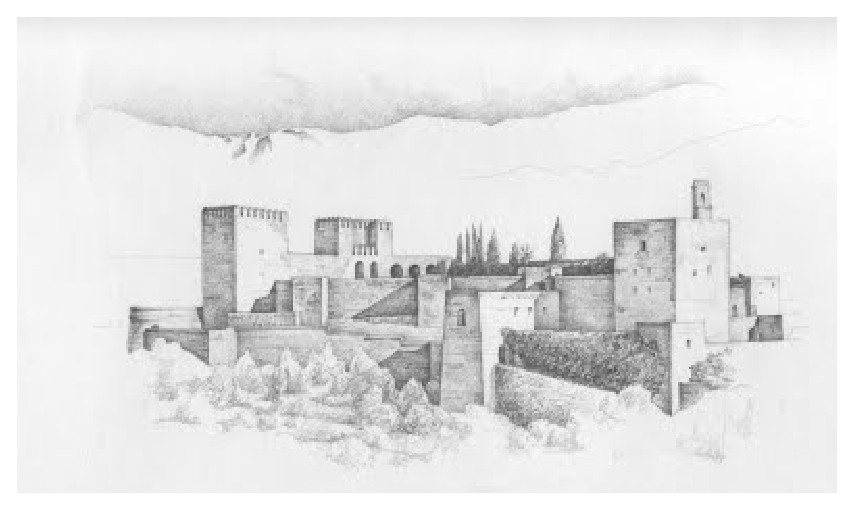
\includegraphics{../imagenes/alhambra-jpg.eps}}}}
 \caption[]{View of the Alhambra}\label{figure 1}
\end{figure}

\vspace{5cm}

{\footnotesize
[1] Author1, Author2 and Author, Journal, Vol (number), Page range(year).
\newline
[2] Author1, Author2 and Author, Journal, Vol (number), Page range(year).
}

\end{document}

